%! TEX root = ../main.tex
% ============================================================
% IMMUTABLE — generated automatically, do not edit this block
%   script          : plotter.py::plot_swell_scatter
%   plot_type       : swell_scatter
%   chapter         : 05
%   panel           : None
%   wind            : None
%   amplitude       : 0.1, 0.2, 0.3
%   frequency       : None
%   probes          : None
%   draft           : True
%
% DATASETS:
%   PROCESSED-20260326-ProbePos4_31_FPV_2-tett6roof-under9Mooring-height100-lowrange
%   PROCESSED-20260327-ProbePos4_31_FPV_2-tett6roof-under9Mooring30-height100-lowrange
%
% SUBFIGURES AVAILABLE:
%   FIGURES/ch05_swell_scatter.pdf
%   FIGURES/ch05_swell_scatter.pdf
%   FIGURES/ch05_swell_scatter.pdf
% ============================================================
\begin{figure}[htbp]
  \centering
  \begin{subfigure}[b]{0.48\linewidth}
    \centering
    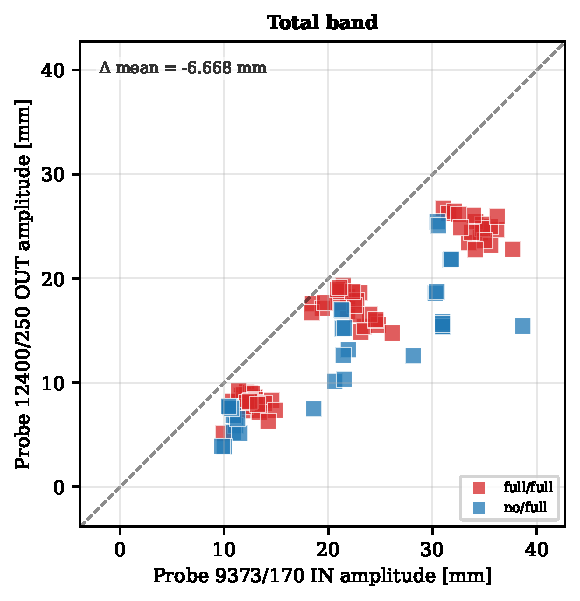
\includegraphics[width=\linewidth]{FIGURES/ch05_swell_scatter.pdf}
    \caption{TODO}
    \label{fig:TODO_1}
  \end{subfigure}
  \hfill
  \begin{subfigure}[b]{0.48\linewidth}
    \centering
    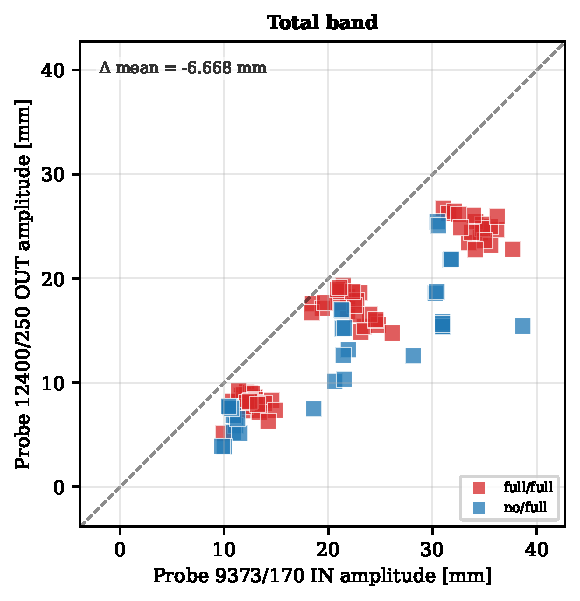
\includegraphics[width=\linewidth]{FIGURES/ch05_swell_scatter.pdf}
    \caption{TODO}
    \label{fig:TODO_2}
  \end{subfigure}
  \hfill
  \begin{subfigure}[b]{0.48\linewidth}
    \centering
    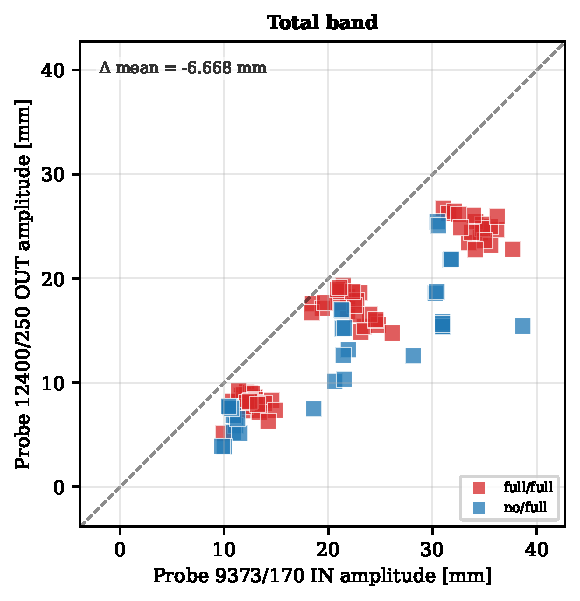
\includegraphics[width=\linewidth]{FIGURES/ch05_swell_scatter.pdf}
    \caption{TODO}
    \label{fig:TODO_3}
  \end{subfigure}
  \caption[Short caption for LOF]{
    % TODO: write caption
  }
  \label{fig:ch05_swell_scatter}
\end{figure}
